\documentclass[a4paper]{article}

\usepackage{caption}
\usepackage{listings}
\usepackage{fancyhdr}
\usepackage[top=3cm,bottom=3cm,left=3cm,right=3cm]{geometry}
\usepackage{color}
\usepackage{amsmath}
\usepackage{graphicx}

\definecolor{dkgreen}{rgb}{0,0.6,0}
\definecolor{gray}{rgb}{0.5,0.5,0.5}
\definecolor{mauve}{rgb}{0.58,0,0.82}

\lstset{frame=tb,
  language=Java,
  aboveskip=3mm,
  belowskip=3mm,
  showstringspaces=false,
  columns=flexible,
  basicstyle={\small\ttfamily},
  numbers=none,
  numberstyle=\tiny\color{gray},
  keywordstyle=\color{blue},
  commentstyle=\color{dkgreen},
  stringstyle=\color{mauve},
  breaklines=true,
  breakatwhitespace=true
  tabsize=3
}

\newcommand{\HRule}{\rule{\linewidth}{0.5mm}}
\pagestyle{fancy}
\lfoot{\small \color{gray}Tom Peerdeman - 10266186}
\cfoot{\thepage}
\rfoot{\small \color{gray}Ren\'e Aparicio Sa\'ez - 10214054}
\lhead{\small \color{gray}Betrouwbaarheids Intervallen}

\begin{document}
\begin{titlepage}
\begin{center}
\textsc{\Large Autonome Mobiele Robots}\\[0.5cm]
\HRule \\[0,4cm]
\textsc{\huge \bfseries NXT - Steering}
\HRule \\[8cm]
\begin{minipage}{0.4\textwidth}
\begin{flushleft}\large
\emph{Auteurs: Tom Peerdeman \& Ren\'e Aparicio Saez}\\
\end{flushleft}
\end{minipage}
\begin{minipage}{0.4\textwidth}
\begin{flushright}\large
\emph{Datum: \today\\\hspace{1cm}}\\
\end{flushright}
\end{minipage}
\end{center}
\end{titlepage}

\section{Kinematica}
Insert plaatje uit opgave hier

\subsection{Kinematica van twee robots}
Robot met twee wielen:\\
$\mathrm{[\dot{x}\; \dot{y}\; \dot{\theta}]^T} = f\mathrm{(l, r, \theta, \varphi_{1}, \varphi_{2})}$\\
\\
De variabelen voor het castor-wiel hoeven niet meegenomen te worden in de functie, omdat het castor-wiel niet gemotoriseerd is. Omdat deze daarom geen invloed uitoefent op de richting of snelheid van het voertuig, kan het castor-wiel gezien worden als een sleepwiel dat in de functie te verwaarlozen valt.\\\\
Robot met drie wielen:\\
$\mathrm{[\dot{x}\; \dot{y}\; \dot{\theta}]^T} = f\mathrm{(l, r, \theta, \varphi_{1}, \varphi_{2}, \varphi_{3})}$\\


\subsubsection{Odometry}
a.De makkelijkste manier om te kijken naar de invloed van de draaisnelheiden van de wielen op de positie en de orientatie is door deze eerst te bepalen in het robot co\"ordinaten stelsel. Dit is makkelijker te bepalen aangezien de robot in dit co\"ordinaten stelsel nooit een snelheid kan krijgen in de y richting door de constraint dat er geen slip aanwezig is.\\
De snelheid in de x richting is ook makkelijk te bepalen. Stel dat alleen wiel 1 draait met snelheid $\varphi_{1}$, aangezien P in het midden ligt van wiel 1 en 2 zal deze zich dus voorbewegen met een snelheid van $\frac{1}{2}r\varphi_{1}$ in de x richting. Aangezien dit ook geldt als alleen wiel 2 draait kunnen we deze optellen als allebei de wielen draaien.
In het geval dat de wielen draaien met snelheden $\varphi_{1}$ en $\varphi_{2}$ zal de robot dus een snelheid krijgen van $\frac{1}{2}r\varphi_{1} + \frac{1}{2}r\varphi_{2}$ in de x richting.\\\\
De rotatie is op een zelfde manier te berekenen. stel dat wiel 1 stil staat en wiel 2 zo draait dat er een positieve snelheid in de x richting ontstaat. In dit geval gaat de robot draaien om het contactpunt van wiel 1. We kunnen zeggen dat wiel 2 rijd op een circkel met radius 2l en als middelpunt het contactpunt van wiel 1. Aangezien we de draaisnelheid weten van wiel 2 kunnen we de rotatiesnelheid van dit wiel berekenen met de volgende formule:\\
$\omega_{1}=\frac{r\varphi_{1}}{2l}$\\
Stel nu dat wiel 1 draait en wiel 2 stilstaat, we krijgen dan ook een rotatie, echter in de andere richting dan eerst.
De formule blijft dus hetzelfde op het feit na dat de draairichting, en dus de rotatiesnelheid negatief wordt:
$\omega_{2}=-\frac{r\varphi_{2}}{2l}$\\
Aangezien de rotatiesnelheid in situatie 1 in het punt P gelijk is aan dat van wiel 2, en in situatie 2 die van wiel 1 kunnen we deze optellen om zo de totale rotatiesnelheid te krijgen in punt P: $\omega=\frac{r\varphi_{1}}{2l}-\frac{r\varphi_{2}}{2l}$\\\\
We weten nu alle benodigde snelheden in robot co\"ordinaten:\\\\
$
\dot{\xi_{R}}
\begin{bmatrix}
\frac{1}{2}r\varphi_{1} + \frac{1}{2}r\varphi_{2} \\
0\\
\frac{r\varphi_{1}}{2l}-\frac{r\varphi_{2}}{2l}
\end{bmatrix}
=
\begin{bmatrix}
\dot{x} \\
\dot{y} \\
\dot{\theta}
\end{bmatrix}_{R}
$
\\\\
We kunnen nu de snelheden omzetten naar wereld co\"ordinaten door de inverse van de rotatiematrix te gebruiken:\\
$
\dot{\xi_{I}}=
R(\theta)^{-1}
\begin{bmatrix}
\frac{1}{2}r\varphi_{1} + \frac{1}{2}r\varphi_{2} \\
0\\
\frac{r\varphi_{1}}{2l}-\frac{r\varphi_{2}}{2l}
\end{bmatrix}
=
R(-\theta)
\begin{bmatrix}
\frac{1}{2}r\varphi_{1} + \frac{1}{2}r\varphi_{2} \\
0\\
\frac{r\varphi_{1}}{2l}-\frac{r\varphi_{2}}{2l}
\end{bmatrix}
$
\\\\\\
b. 1. De precisie van de inschatting verbetert naarmate de $\Delta t$ afneemt. Dit komt omdat als de positie net geschat is en de robot zich beweegt, de positie voor een tijd van $\Delta t$ incorrect is. Als $\Delta t$ afneemt zal de precisie van de gemiddelde inschatting dus toenemen.\\\\
2. De rotatie snelheid in robot co\"ordinaten is uitgewerkt in opgave a. Aangzien de rotatiematrix echter niks doet met deze waarde is deze waarde dus gelijk aan de rotatiesnelheid in het wereldco\"ordinaten stelsel. De rotatiesnelheid is dus:\\
$w(t) = \omega=\frac{r\varphi_{1}}{2l}-\frac{r\varphi_{2}}{2l}$\\\\
3. De v vector heeft twee elementen: de snelheid in de x richting en de snelheid in de y richting. We kunnen de v vector dus berekenen door de x en y snelheid in robot co\"ordinaten te vermenigvuldigen met een niet homogene rotatiematrix over de hoek $-\theta$:\\\\
$
\vec{v}=
\begin{bmatrix}
\dot{x} \\
\dot{y}
\end{bmatrix}
=
\begin{bmatrix}
cos(-\theta) & sin(-\theta)\\
-sin(-\theta) & cos(-\theta)
\end{bmatrix}
\begin{bmatrix}
\frac{1}{2}r\varphi_{1} + \frac{1}{2}r\varphi_{2} \\
0
\end{bmatrix}
$

\section{Steering Experimenten}

\subsection{Theorie (a)}
De robot moet onderscheidt kunnen maken tussen twee basis bewegingen. Een rechte lijn en een bocht maken (deel van de vorm van een cirkel).\\
\\
De theorie voor een rechte lijn rijden is eenvoudig. De robot moet weten wat de af te leggen afstand $\psi$ is en met welke snelheid $\varphi$ hij deze moet gaan afleggen. Als deze waarden bekend zijn, kan bepaald worden hoeveel tijd de wielen dit moeten uitvoeren en kan een rechte lijn gereden worden.\\
\\
Een bocht maken is wat minder eenvoudig. Hiervoor moet bekend zijn wat de afstand van elk wiel tot aan het middelpunt van de robot is $l$ (deze afstand is voor elk gemotoriseerd wiel hetzelfde). Daarnaast moet bekend zijn wat de radius $r$ van de cirkel is waar omheen gereden moet worden. Deze radius wordt bepaald vanaf het middelpunt $P$ van de robot tot aan het middelpunt van de cirkel die de bocht definieert. Er moet ook bekend zijn hoeveel graden $\alpha$ er moet worden gedraaid. De snelheid voor de wielen moet vervolgens per wiel berekend worden. De snelheid $\varphi_1$ voor het wiel aan de buitenkant van de bocht wordt geleverd. Om de snelheid voor het tweede wiel te bepalen moet eerst bepaald worden wat de afstand is die elk wiel moet afleggen. Dit wordt als volgt bepaald:\\\\
voor het wiel aan de buitenkant van de bocht:
$s_1 = \frac{2\pi(r + l)}{360}\alpha$\\
voor het wiel aan de binnenkant van de bocht:
$s_2 = \frac{2\pi(r - l)}{360}\alpha$\\\\
Vervolgens kan de tijd $t$ bepaald worden door de afstand voor het buitenste wiel te delen door de meegeleverde bijbehorende snelheid. Deze berekende $t$ geeft aan hoelang het wiel moet draaien. Als $t$ bekend is kan ook de snelheid voor het binnenste wiel worden berekend. $\varphi_2=\frac{s_2}{t}$

\subsection{Feedback  (b)}
Als bewegingen zijn uitgevoerd kan nagegaan worden of dit juist is verlopen. Door tijdens het uitvoeren van een beweging bij te houden of de wielen de juiste afstand hebben afgelegd kan bepaald worden of er afgeweken is van de oorspronkelijke waarde. Als deze waarde afwijkt van de oorspronkelijke waarde moet hiervoor gecompensserd worden bij de volgende beweging. Dit kan worden gedaan door de afstand die teveel of te weinig is afgelegd, van de volgende beweging af te halen.

\subsection{Implementatie (c)}
\subsubsection{Rechte lijn}
De implementatie voor de rechte lijn is vrij voor de hand liggend. Beide wielen krijgen dezelfde power mee. Voor de afstand is echter gekozen om aan te geven hoeveel graden de wielen moeten draaien. Dit is gedaan omdat de call naar de NXT-robot niet kan werken met afstanden maar wel met omwentelingen aangegeven in het aantal graden.
\begin{lstlisting}[caption=Rechte lijn, label=lst:line, numbers=left]
function NXTLine(phi, wentels)
NXT_SetOutputState(MOTOR_B, phi, true, true, 'SPEED', 0, 'RUNNING', wentels, 'dontreply');
NXT_SetOutputState(MOTOR_C, phi, true, true, 'SPEED', 0, 'RUNNING', wentels, 'dontreply');
\end{lstlisting}
\subsubsection{Bocht}
Voor de bocht moeten er meerdere berekeningen gedaan worden. De theorie blijft van kracht, er vormt zich echter een probleem voor de tijdseenheid. De snelheid die meegegeven wordt aan de functie, is niet het aantal rotaties/toeren per minuut maar de power die de motor levert. Echter blijkt dat het verband tussen de power ten opzichte van het aantal toeren per minuut lineair is. Dit betekent dat de vreemde snelheids eenheid, namelijk de power, geen invloed heeft op het berekenen van de tijd. De tijd wordt echter van de waarde afstand per power. Omdat continu met dezelfde eenheden wordt gewerkt wordt uiteindelijk de eenheid voor de snelheid van het tweede wiel gewoon power. Vervolgens wordt de afstand die afgelegd moet worden omgerekend naar het aantal graden dat elk wiel moet draaien, zodat dit aan de call kan worden meegegeven. Tenslotte moet er bekeken worden welke kant opgedraaid moet worden, links of rechts. Aan de hand van een if else statement kan hier op worden gecontroleerd.
\begin{figure}[h]
	\centering
	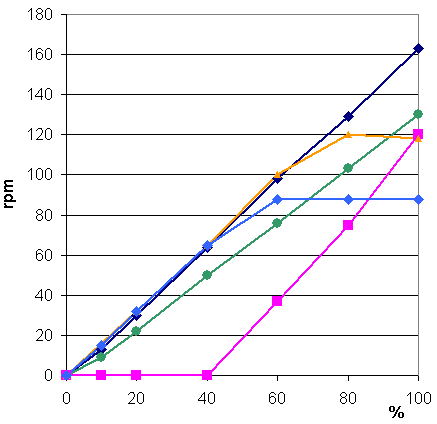
\includegraphics[width=0.6\textwidth]{imgs/lineair.png}
	\caption{Lineair verband, donkerblauw is voor een ongeladen motor, 9V NXT motor\protect\footnotemark}
	\label{fig:lineairverband}
\end{figure}
\footnotetext{Original source: http://www.philohome.com/nxtmotor/nxtmotor.htm}
\\\\
\begin{lstlisting}[caption=Bocht, label=lst:bocht, numbers=left]
function NXTBocht(radius, alpha, phi1, richting)
s1 = (2*pi*(radius+5.85))/360 * alpha;
s2 = (2*pi*(radius-5.85))/360 * alpha;
t = s1 / phi1;
phi2 = s2/t;
wentel1 = s1/17.593 * 360;
wentel2 = s2/17.593 * 360;
% bocht naar rechts
if richting
NXT_SetOutputState(MOTOR_C, phi1, true, true, 'SPEED', 0, 'RUNNING', wentel1, 'dontreply');
NXT_SetOutputState(MOTOR_B, phi2, true, true, 'SPEED', 0, 'RUNNING', wentel2, 'dontreply');
% bocht naar links
else
NXT_SetOutputState(MOTOR_C, phi2, true, true, 'SPEED', 0, 'RUNNING', wentel2, 'dontreply');
NXT_SetOutputState(MOTOR_B, phi1, true, true, 'SPEED', 0, 'RUNNING', wentel1, 'dontreply');
end
\end{lstlisting}
\subsubsection{Meerdere bewegingen}
Tot slot moet er voor gezorgd worden dat er meerdere bewegingen achter elkaar kunnen worden uitgevoerd. Hiervoor moet per beweging worden gewacht totdat deze klaar is. Hier wordt op gecheckt door de status van de motors te bekijken. Zodra deze geen power meer leveren wordt het signaal 'IDLE' afgegeven. Zodra dit signaal is ontvangen kan een eventueel volgende beweging worden uitgevoerd.
\begin{lstlisting}[caption=Meerdere moves, label=lst:moves, numbers=left]
while(1)
    outB = NXT_GetOutputState(MOTOR_B);
    outC = NXT_GetOutputState(MOTOR_C);
    if strcmp(outB.RunStateName, 'IDLE') && strcmp(outC.RunStateName, 'IDLE')
        break
    end
end
\end{lstlisting}
\subsubsection{feedback}
Error compensatie bij rechte lijnen lijkt erg vanzelfsprekend. Er wordt bekeken hoeveel graden de motor voor de omwenteling heeft gemaakt voor de beweging, en hoeveel omwentelingen er gedaan zijn na de beweging. Het verschil tussen deze twee waarden zou gelijk moeten zijn aan de oorspronkelijk ingevoerde waarde voor de omwentelingen. Het verschil hiertussen is de error. Om zeker te weten dat er geen error compensatie wordt uitgevoerd van bewegingen uit een oud programma, moet deze worden geinitialisserd bij het starten van de bewegingen. 
\begin{lstlisting}[caption=Error compensatie bij een lijn, label=lst:lineerror, numbers=left]
function NXTLinet(phi, wentels)
global error
outB = NXT_GetOutputState(MOTOR_B);
beforeB = outB.TachoCount;
outC = NXT_GetOutputState(MOTOR_C);
beforeC = outC.TachoCount;
NXT_SetOutputState(MOTOR_B, phi, true, true, 'SPEED', 0, 'RUNNING', wentels-error(1), 'dontreply');
NXT_SetOutputState(MOTOR_C, phi, true, true, 'SPEED', 0, 'RUNNING', wentels-error(2), 'dontreply');
while(1)
    outB = NXT_GetOutputState(MOTOR_B);
    outC = NXT_GetOutputState(MOTOR_C);
    if strcmp(outB.RunStateName, 'IDLE') && strcmp(outC.RunStateName, 'IDLE')
        break
    end
end

outB = NXT_GetOutputState(MOTOR_B);
afterB = outB.TachoCount;
outC = NXT_GetOutputState(MOTOR_C);
afterC = outC.TachoCount;
diffB = abs(afterB-beforeB)+error(1);
diffC = abs(afterC-beforeC)+error(2);
error = [diffB-wentels diffC-wentels];
\end{lstlisting}
Uit experimenten blijkt echter dat de berekende error-waarden erg fluctueren. Bij dezelfde gereden afstand met dezelfde snelheid verschilt de error tussen 20 en 60 graden (gemeten door de TachoCount). Er is dus geen verband tussen afstand en error te vinden, of tussen snelheid en error. Zonder te compenseren voor deze error-waarden worden betere resultaten bereikt. Dus is besloten voor de bocht geen error-compensatie door middel van TachoCount te maken.
\end{document}
